% This is samplepaper.tex, a sample chapter demonstrating the
% LLNCS macro package for Springer Computer Science proceedings;
% Version 2.20 of 2017/10/04
%
\documentclass[runningheads]{llncs}
%
\usepackage{graphicx}
\usepackage{titlesec}

\setcounter{secnumdepth}{4}
% Used for displaying a sample figure. If possible, figure files should
% be included in EPS format.
%
% If you use the hyperref package, please uncomment the following line
% to display URLs in blue roman font according to Springer's eBook style:
% \renewcommand\UrlFont{\color{blue}\rmfamily}

\begin{document}
%
\title{Classification of COVID-19 based on CT images obtained from scientific papers.}
%
\titlerunning{Classification of COVID-19 based on CT images}
% If the paper title is too long for the running head, you can set
% an abbreviated paper title here
%
\author{Mikołaj Najda\inst{1}\and
Dominik Ćwikowski\inst{1}}
%
\authorrunning{M. Najda, D. Ćwikowski}
% First names are abbreviated in the running head.
% If there are more than two authors, 'et al.' is used.
%
\institute{\inst{1}Wrocław University of Science and Technology, 
\email{276928@student.pwr.edu.pl}[Mikołaj Najda]}
%
\maketitle              % typeset the header of the contribution 

%
\begin{abstract}
Abstrakt napiszemy po zrobieniu całej pracy - 15--250 words.

\keywords{COVID-19 \and RASNet \and Machine Learning \and Classification.}
\end{abstract}
%
%
%
\section{Introduction}
The COVID-19 outbreak has demonstrated the significant impact that the Internet of Things (IoT) and artificial intelligence (AI) fields have had on the healthcare industry, including the ability to assist with health monitoring, quarantine e-tracking, detection and diagnosis \cite{ITcovidReview}. Rapid developments in machine learning have sparked new ideas among researchers \cite{MLDLcovidReview}. AI-based models have been used to forecast the performance of illnesses by analyzing COVID-19-related symptoms, such as throat pain, immunity status, and diarrhoea \cite{covidForecasting}. Sentiment analysis of public opinions has also been performed based on tweets, using models such as SFODLD-SAC for data preprocessing and CRNN for sentiment analysis and classification \cite{sentimentTweets}. Image classification, a task widely developed by deep learning researchers, has been used in conjunction with chest X-rays and computed tomography (CT) scans to detect lung changes caused by the virus. Machine learning techniques, such as Convolutional Neural Networks (CNNs), have shown their potential in these image-related solutions. The workflow for deploying deep learning-based tools typically includes gathering data, pre-processing (e.g. normalization, resizing, and segmentation), applying transfer learning or neural network architecture from scratch, setting up the classification classes based on the problem and data, and choosing appropriate metrics to evaluate model performance \cite{MLDLimageReview}.
\newline
\indent
Convolution Neural Network (CNN) is the deep learning technique that enables achieving astonishing results in tasks related to image classification. It allows performing these tasks based on focusing on the relationship of the nearby pixels (contextual information). The general model of CNN is built with four components: convolution layer, pooling layer, activation function and fully connected layer \cite{CNNexplanation}. The approach with CNN helps to avoid complicated feature engineering in medical image classification tasks. CNN-based transfer learning method seems to be one of the best choices for dealing with a small amount of data. By unfreezing the later layers, fine-tuning and omitting to overfit the model for a particular task is possible \cite{CNNmedicalimageclassification}.
\newline
\indent
Transfer learning involves applying a pre-trained model on large datasets to a target model. Due to the lack of large medical image datasets which are properly labelled by professionals the transfer learning approach gained popularity. It allows for improving the generalization of the model, even if the dataset that the model was pre-trained on is not related of any kind to data for the particular problem. The pre-trained model is already learned to recognize features such as edges or corners which are common in every image. It is hard not to come across scientific papers about medical image classification where the authors did not try to apply this method \cite{TransferLearningCOVID19}.
\newline
\indent
Self-supervised learning is a form of semi-supervised learning, it tries to learn important correlations between extracted features of input unlabelled data, providing learning by solving auxiliary tasks. Pretext tasks are a type of auxiliary tasks which are performed to learn a model to extract useful features from images. Those problems may include predicting the missing part or rotation of an image. This approach allows using the large unlabelled datasets as a supportive way to pre-train the model and achieve better results on a target problem if only the pretext tasks are successfully designed \cite{SelfSupervisedLearnig}.
\newline
\indent
It is worth diving into state-of-art machine learning methods in the case of medical image classification, which are being superseded by neural networks. Although, sometimes there is no need to use power-consuming deep learning approaches and certainly not without trying methods like Principal Component Analysis (PCA) or Support Vector Machine (SVM).  
\newline
\indent
PCA's purpose is the reduction of the large dimensionality of observed variables to smaller, essential independent variables. It identifies patterns in a dataset by finding a set of new variables called principal components that contain the most significant information in the original data. It is considered a powerful tool for feature extraction from large datasets like an image. One of the uses of PCA is medical image classification \cite{PCA1}. However, nowadays researchers started to apply PCA along with neural networks to enhance the model's accuracy and reduce computation time. The authors have shown that the use of PCA with deep learning solutions can outperform comparative methods \cite{PCA2}.  
\newline
\indent
The SVM classifier is used by many researchers in medical image classification tasks. SVMs work by finding the best boundary or plane that separates data points of different classes in a dataset. The algorithm identifies the data closest to the set line or plane which is called the support vector and it is used to optimize a boundary or a plane. The kernel is a function used for mapping the input data into higher-dimensional feature space, the one commonly used in image classification is the Gaussian radial basis function (RBF) \cite{SVM1,SVM2}.
\newline
\indent
The covid-19 outbreak gathered researchers who started developing deep learning tools in order to help diagnosticians with detecting lung pathologies caused by the virus from CT scans. A weakly-supervised framework for classification and lesion localization was presented. Weak supervision means that only image-level labels (virus positive or negative in this example) are used during training instead of pixel-level labels such as edges, and shapes of the region of interest (ROI). They have proposed an approach that contains three main steps: a feature extractor as a pre-trained and then fine-tuned CNN, a lesion localization module to identify potential lesion regions in the scans using a binary classifier and a fully connected network as a classification model.
The framework achieved a better result (0.90) than classic approaches like RBF SVM, linear SVM or Random Forest, respectively (0.72, 0.75, 0.78) but give way to human expert (0.97). However, new approaches can enhance the classification tasks in the future and can become robust tools for professionals to improve their performance \cite{WeaklyFramework}.
\newline
\indent
One group of researchers tried to develop the best tool for COVID-19 classification based on CT images. However, back in 2020, publicly available datasets were limited, so they gathered images from articles. The main question that arose was whether the images downloaded from the papers were still valuable in any pathology classification, given the loss in image quality and only selected slices. The authors of the challenge assured that the usability of the dataset was confirmed by an experienced radiologist who had been working with COVID-19 cases since the start of the pandemic \cite{zhao2020COVID-CT-Dataset}. They developed a sample-efficient deep learning method to demonstrate the usability of the low-sample dataset and besides big differences in target data (CT images) and data of pre-trained neural networks (animals, furniture) investigated transfer learning and self-supervised learning methods. In order to evaluate the classification task, they decided to test transfer learning based on pre-trained models on datasets such as ImageNet \cite{ImageNet} and Lung Nodule Malignancy (LNM). A few different networks were applied to check the performance for the particular problem, the VGG16, ResNet18, ResNet50, DenseNet-121, DenseNet-169, EfficientNet-b0, and EfficientNet-b1 were evaluated. According to the knowledge of having a relatively small dataset, the light-weight neural network architecture was designed \cite{he2020sample}. 
They used batch normalization, and binary cross-entropy as the loss-function, hyperparameters were tuned on the validation set as experimental settings and a different data augmentation for two approaches were implemented. They have shown results in three metrics: Accuracy, F1-score and AUC.
They achieved the highest scores for DenseNet-169, F1-score and AUC metrics for the network that was pre-trained first on ImageNet, then on LMN respectively (0.82, 0.89), and the highest Accuracy (0.83) for the network that was pre-trained only on the ImageNet dataset. 
The self-supervised approach yielded the highest Accuracy, F1-score and AUC using the DenseNet-169, respectively (0.86, 0.85, 0.94) with the following steps: pre-train on ImageNet, perform Self-Supervised Learning (SSL) on Lung Nodule Analysis (LUNA) dataset without using labels of LUNA, then perform SSL on COVID19-CT without using labels of COVID19-CT and at the end fine-tune on COVID19-CT using labels. However, the authors evaluated the self-supervised learning using the data from the LUNA database and they did not include selected data in their GitHub, we took this fact into consideration during work with the problem and decided to... .  
\newline
\indent
This paper presents two approaches to dealing with the dataset: one based on the authors' solution and the second on k-fold cross-validation to analyze the impact of choosing the preferred data split for n $<$ 1000 \cite{kfoldcrossvalidationN1000}. Standard machine learning methods such as Principal Component Analysis (PCA), and Support Vector Machine (SVM) were used and deep learning solutions were evaluated, all of the results are shown in this work. However, machine learning solutions in the medical imaging field continue to evolve, and each year new models and algorithms are developed. It is important to keep in mind that, especially in the healthcare industry, the accuracy of any solution must be high.

\section{Proposed experimental design}
%Plan eksperymentu
%Sformułowanie tzw. research questions, czyli pytań, na które mają odpowiedzieć prowadzone badania.
%Przedstawienie dokładnych celów eksperymentów.
%Opis wybranych zestawów danych (liczba klas, cech, instancji).
%Dokładny opis planu eksperymentu z naciskiem na wykorzystywany protokół badawczy.
%Opis środowiska eksperymentalnego.
\subsection{Research questions}

\begin{itemize}
  \item Is it possible to make a machine learning model that is able to classify medical images based on low-quality data obtained from scientific articles?
  \item Will the state-of-art approaches outperform deep learning methods?
  \item How really the right way of splitting the data will influence the performance of methods presented by the authors of the challenge?
  \item What the deep learning model took into consideration when predicting the class of image?
  \item Does the data augmentation improve the model generalization?
\end{itemize}

\subsection{Precise experiment purpose}

The target of this work is to test the best deep learning model shown in \cite{he2020sample}, and compare its performance with the results given by PCA, SVM and proposed, simple CNN. However, the test will be separated at the data preparation step. Once we test the data split proposed by the authors then we are going to do an approach with k-fold cross-validation. Ultimately, the results will be compared and discussed.

\subsection{Dataset}

The data for the training set were prepared as part of the Challenge - Grand Challenge on COVID-19 diagnosis from CT images. The images of COVID-19 positive were taken from scientific papers from medRxiv and bioRxiv publications, and the COVID-19 negative from sources such as the MedPix database and PubMed Central. Example CT scans from individuals who have been infected with the virus with visible lesions are shown in (Figure \ref{covidPositive}) and healthy individuals are presented in (Figure \ref{covidNegative}). Information about COVID-related and non-COVID data is presented in (Table \ref{imageDetails}).
\newline

Key notes about data:
\begin{itemize}
  \item The corpus of test and validation images was procured from an external source featuring computed tomography (CT) images that were not acquired via paper downloads. Notwithstanding, the authors solely furnished the data distribution pertaining to the training, validation, and testing sets based on the images obtained from the papers, as demonstrated in Table \ref{imageDistributionAuthors}. Preventing the proper comparasion to their's results shown in the paper.
  \item Utilizing a data split, as implemented by the authors, may not be optimal when dealing with a relatively small number of images (n $<$ 1000), as suggested in \cite{kfoldcrossvalidationN1000}. Given that each data example is crucial for effectively training a model, we opted to utilize k-fold cross-validation instead of the holdout method in our approach, to mitigate the potential for model overfitting.
  \item Due to the small dataset, data augmentation has been performed using different random affine transformations such as random cropping with a scale of 0.5, horizontal flip as well as colour jittering with random contrast and random brightness with a factor of 0.2. However additional augmentations were added for the self-supervised approach.
\end{itemize}

\begin{table}[h]
\label{imageDetails}
\centering
\caption{Dataset details.}
\begin{tabular}{c|c}
\cline{1-2}
 COVID-19 & Number \\ \cline{1-2}
 Positive & 349 \\ \cline{1-2}
 Negative & 397  \\ \cline{1-2}
\end{tabular}
\end{table} 

\begin{figure}[h]
\centering
{
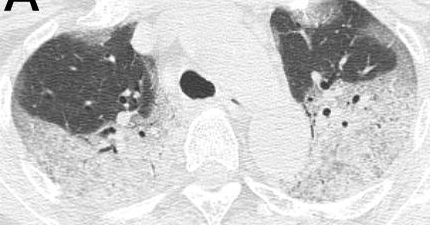
\includegraphics[width=0.40\textwidth]{imagesDatasetSection/covid1.png}
}
\quad
{
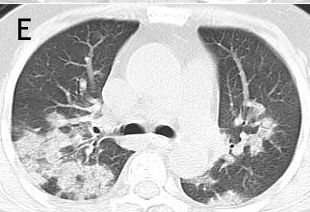
\includegraphics[width=0.30\textwidth]{imagesDatasetSection/covid2.png}
}
\label{covidPositive}
\caption{CT COVID Positive.}
\end{figure}

\begin{figure}[h]
\centering
{
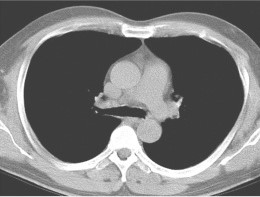
\includegraphics[width=0.30\textwidth]{imagesDatasetSection/noncovid1.jpg}
}
\quad
{
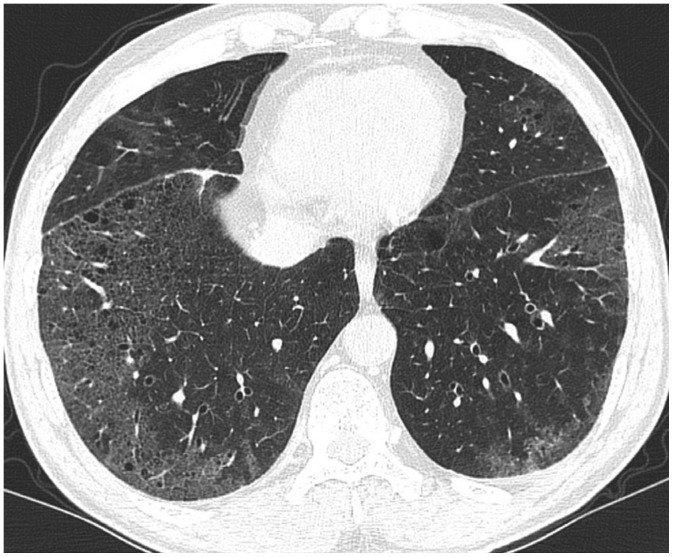
\includegraphics[width=0.27\textwidth]{imagesDatasetSection/noncovid2.jpg}
}
\label{covidNegative}
\caption{CT COVID Negative.}
\end{figure}

\begin{table}[h]
\label{imageDistributionAuthors}
\centering
\caption{Images distribution.}
\begin{tabular}{c|c|c|c}
\cline{1-4}
Type & NonCOVID-19 & COVID-19 & Total \\ \cline{1-4}
training & 234 & 191 & 425\\ \cline{1-4}
validation & 58 & 60 & 118\\ \cline{1-4}
test & 105  & 98 & 203\\ \cline{1-4}
\end{tabular}
\end{table} 


\subsection{Research protocol}

The study will acquire the dataset for training and testing the models through the authors' approach or k-fold cross-validation. Further, the images will be subjected to augmentation to produce four distinct datasets. The performance of the best model using the authors' approach will be compared against other state-of-the-art methods, including our proposed CNN. Common metrics such as F1-score, confusion matrix, or ROC Curve will be used to evaluate the results. Moreover, visualization will be attempted to explain the factors influencing the best model's prediction of image labels.

\subsection{Description of the experimental environment}
The project will be written in Python programming language, with Jupyter Notebook as the preferred Integrated Development Environment on the Google Colab cloud-based service that provides free access to GPU resources. PyTorch and scikit-learn (sklearn), widely used Python modules for machine learning, will be utilized for the development of the CNN and other state-of-the-art machine learning approaches.

\section{Methods and evaluation}

\section{Results}
%MOZE SAMI WYKORZYSTAMY Grad-CAM do wizualizacji wynikow/wyglada ciekawie

\section{Summary}


%
% ---- Bibliography ----
%
% BibTeX users should specify bibliography style 'splncs04'.
% References will then be sorted and formatted in the correct style.
%
% \bibliographystyle{splncs04}
% \bibliography{mybibliography}
\begin{thebibliography}{99.}

\bibitem{ITcovidReview}
Mondal S, Mitra P.: The Role of Emerging Technologies to Fight Against COVID-19 Pandemic: An Exploratory Review. Trans Indian Natl Acad Eng., 99--110 (2022)

\bibitem{MLDLcovidReview}
Showmick Guha Paul, Arpa Saha, Al Amin Biswas, Md. Sabab Zulfiker, Mohammad Shamsul Arefin, Md. Mahfujur Rahman, Ahmed Wasif Reza: Combating Covid-19 using machine learning and deep learning: Applications, challenges, and future perspectives. Array, Volume 17 (2023)

\bibitem{covidForecasting}
Rehman MU, Shafique A, Khalid S, Driss M, Rubaiee S.: Future Forecasting of COVID-19: A Supervised Learning Approach. Sensors (Basel), (2021)

\bibitem{sentimentTweets}
Alkhaldi, Nora A., Yousef Asiri, Aisha M. Mashraqi, Hanan T. Halawani, Sayed Abdel-Khalek, and Romany F. Mansour: Leveraging Tweets for Artificial Intelligence Driven Sentiment Analysis on the COVID-19 Pandemic. Healthcare 10, (2022)

\bibitem{MLDLimageReview}
Priya Aggarwal, Narendra Kumar Mishra, Binish Fatimah, Pushpendra Singh, Anubha Gupta, Shiv Dutt Joshi: COVID-19 image classification using deep learning: Advances, challenges and opportunities. Computers in Biology and Medicine, Volume 144 (2022)

\bibitem{zhao2020COVID-CT-Dataset}
Zhao, Jinyu and Zhang, Yichen and He, Xuehai and Xie, Pengtao: COVID-CT-Dataset: a CT scan dataset about COVID-19. arXiv preprint arXiv:2003.13865, (2020)

\bibitem{he2020sample}
He, Xuehai and Yang, Xingyi and Zhang, Shanghang, and Zhao, Jinyu and Zhang, Yichen and Xing, Eric, and Xie, Pengtao: Sample-Efficient Deep Learning for COVID-19 Diagnosis Based on CT Scans. medrxiv, (2020)

\bibitem{CNNexplanation}
Sakshi Indolia, Anil Kumar Goswami, S.P. Mishra, Pooja Asopa: Conceptual Understanding of Convolutional Neural Network- A Deep Learning Approach. Procedia Computer Science 132, 679--688 (2018)

\bibitem{CNNmedicalimageclassification}
Yadav, S.S., Jadhav, S.M.: Deep convolutional neural network based medical image classification for disease diagnosis. J Big Data 6, Volume 113 (2019)

\bibitem{TransferLearningCOVID19}
Kevser Sahinbas, Ferhat Ozgur Catak: Transfer learning-based convolutional neural network for COVID-19 detection with X-ray images. Data Science for COVID-19, 451-466 (2021)

\bibitem{SelfSupervisedLearnig}
Kriti Ohri, Mukesh Kumar: Review on self-supervised image recognition using deep neural networks. Knowledge-Based Systems, Volume 224, (2021)

\bibitem{PCA1}
Nandi, Dibyadeep Ashour, Amira S. Samanta, Sourav Chakraborty, Sayan Salem, Mohammed Abdel-Megeed Mohammed Dey, Nilanjan: Principal Component Analysis in Medical Image Processing: A Study. International Journal of Image Mining, 45-64 (2015)

\bibitem{PCA2}
Mateen, Muhammad Wen, Junhao Nasrullah, Dr Song, Sun Huang, Zhouping: Fundus image classification using VGG-19 architecture with PCA and SVD. Symmetry, (2018)

\bibitem{SVM1}
Khachane, Monali: Organ-Based Medical Image Classification Using Support Vector Machine. International Journal of Synthetic Emotions, 18-30 (2017)

\bibitem{SVM2}
Jair Cervantes, Farid Garcia-Lamont, Lisbeth Rodríguez-Mazahua, Asdrubal Lopez: A comprehensive survey on support vector machine classification: Applications, challenges and trends,
Neurocomputing, Volume 408, 189-215 (2020)

\bibitem{WeaklyFramework}
X. Wang et al.: A Weakly-Supervised Framework for COVID-19 Classification and Lesion Localization From Chest CT. IEEE Transactions on Medical Imaging, vol. 39, no. 8, pp. 2615-2625 (2020)

\bibitem{kfoldcrossvalidationN1000}
Baeldung on CS, \url{https://www.baeldung.com/cs/train-test-datasets-ratio}. Last accessed 19
March 2023

\bibitem{ImageNet}
J. Deng, W. Dong, R. Socher, L. -J. Li, Kai Li and Li Fei-Fei: ImageNet: A large-scale hierarchical image database. IEEE Conference on Computer Vision and Pattern Recognition, (2009)

\bibitem{LearningCurves}
Machine Learning Mystery, \url{https://machinelearningmastery.com/}. Last accessed 28
May 2023

\end{thebibliography}
\end{document}
